\section{Introduction}
%Wireless signals, such as WiFi and the radio frequency (\RF), have emerged as a cheap yet powerful medium for information sensing. By
%measuring how the wireless signal is affected by surrounding objects and human activities, tasks like gait identification~\cite{}, gesture
%recognition~\cite{}, activity recognition~\cite{}, and vital sign monitoring~\cite{} can be possible.
%
%
%The desire for employing wireless signals for sensing could date back to the 19th century  for the discovery of X-rays for object
%recognition~\cite{} and the development of military radar and sonar systems for tracking large metallic objects in open
%spaces~\cite{Charles Samuel Franklin 's development of first practcial radar}. These sensing systems, however, have to rely on expensive specialize hardware and be operated by professionals, which thus put they out of the reach of ordinary people.
%
%
%Recently, it has been shown that wireless sensing built upon consumer-grade devices such as smartphones and wireless routers can be used to
%precisely track human activities in an indoor environment. Such technology has the advantages of being low-cost as it requires as few as
%two wireless routers to operate, not requiring instrumenting the user, being less privacy intrusive compared to other infrastructure-based
%solutions like video-based solutions~\cite{}, and is safer to use on a regular basis compared to other alternatives like X-rays~\cite{}. It
%offers an inexpensive way for bringing activity sensing into everyday life -- which not only makes ever sensing a tantalizing reality but
%could also open up new possibilities for innovative applications.
%
%
%As we will show in this article, while there are still many challenges ahead, consumer-grade wireless sensing has moved from a research
%niche to a mainstream activity. This is, in fact, a dynamic field looking at subjects as diverse as smart-home personalization~\cite{} and
%fall monitoring~\cite{} to emotion detection~\cite{}. In this article we aim to demystify this promising technique, outline the challenges
%it is facing, and show that this is a trustworthy and exciting research direction.
%
%
%
%
%The remainder of this article is structured as follows. We first give an intuitive view for the wireless sensing working mechanism  in
%Section~\ref{sec:mechanism}. \FIXME{We then describe xx, bla bla...}. We discuss the challenges and limitations for wireless sensings, as
%well as open research directions in Section xx before we summarise and conclude in Section \FIXME{xx}.

Wireless signals, such as WiFi, the radio frequency (\RF) and acoustical sounds, have emerged as a powerful medium for information sensing.
By measuring how the wireless signal is affected by surrounding objects and human activities, tasks like localization~\cite{Arraytrack,
Tagoram}, activity recognition~\cite{Wang2015Understanding, wang2016human}, and material identification~\cite{Tagscan, LiquID, zhao2018rf}
could be possible.


The history for using wireless signals for sensing dates back to the 19th century  for the discovery of X-rays for object
recognition~\cite{Suzuki1996} and the development of military radar and sonar systems for tracking large metallic objects in open
spaces~\cite{Au1988Sonar}. These sensing systems, however, have to rely on expensive specialized hardware and be operated by professionals, which
thus put them out of the reach of ordinary people.


Recently, it has been shown that wireless signals generated by consumer-grade devices such as smartphones and wireless routers can be used
to precisely track objects and human activities in an indoor environment, as shown in Fig.~\ref{fig:scenarios}. Such technology has the advantages of being low-cost as it
requires as few as two wireless routers to operate, not requiring instrumenting the user, being less privacy intrusive compared to other
infrastructure-based solutions like video-based solutions~\cite{Cruz2015Quantification}, and is safer to use on a regular basis compared to
other alternatives like X-rays~\cite{De2013B}. It is an inexpensive solution for offering sensing capabilities into everyday life, making
ever sensing a tantalizing reality.

As we will show in this article, while there are still many challenges ahead, consumer-grade wireless sensing has moved from a research
niche to a mainstream activity. This is, in fact, a dynamic field looking at subjects as diverse as smart-home personalization~\cite{vasisht2016decimeter} and
fall monitoring~\cite{wang2017wifall} to emotion detection~\cite{Zhao2017Emotion} and vital sign monitoring~\cite{Smart-homes}. In this article we aim to demystify this promising
technique, outline the challenges it is facing, and show that this is a trustworthy and exciting research direction.


\begin{figure} [t!]
\centering       
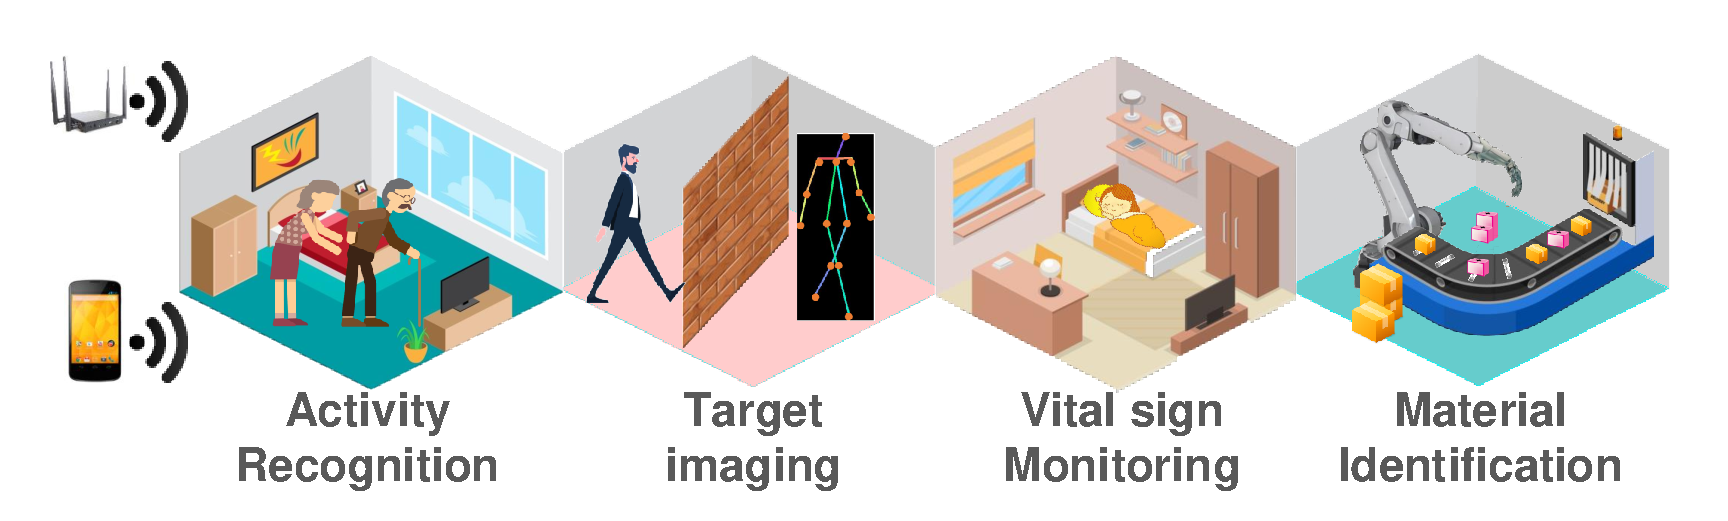
\includegraphics[width=0.5\textwidth]{figures/scenarios.pdf}                
\caption{Examples of wireless sensing.}
\label{fig:scenarios}
\end{figure}

%The remainder of this article is structured as follows. We first give an intuitive view for the wireless sensing working mechanism  in
%Section~\ref{sec:mechanism}. \FIXME{We then describe xx, bla bla...}. We discuss the challenges and limitations for wireless sensings, as
%well as open research directions in Section xx before we summarise and conclude in Section \FIXME{xx}.


%
%The development of wireless devices has resulted in numerous wireless sensing technologies which enable a variety of applications such as
%indoor navigation, smart homes, fitness tracking and security check. In recent years, especially non-contact wireless sensing has attracted
%much attention from both the research community and the industry, due to its convenience of without instrumenting user's body. Many
%researches have answered how to identify object's location, shape, material, behavior, etc. The basic idea of these designs is to utilize
%signal processing to construct a mapping pattern or theoretical relationship between the target information and the signal characteristics.
%
%To turn these designs into practical systems, series challenges need to be tackled. Typically, (i) the defects of cheap devices can lead to
%nonnegligible error of signal information~(phase), (ii) environmental changes can alter the regular signal patterns, and (iii) multi-path
%effect would greatly reduce the estimation resolution of some fundamental parameters for sensing. These always make the system performance
%extremely poor. To address these issues, many efforts has been made, including: (i) calibrating the inaccurate phase information through
%comparing with it with a real value obtained in advance, (ii) canceling background noise using signals from multiple links, and (iii)
%improving the resolution of parameter estimation by splicing bandwidth or constructing virtual array. Nowadays, with the popularity of
%artificial intelligence, deep learning technology is gradually integrated into signal processing to extract more complex and effective
%features for sensing task. This drives great success in wireless sensing applications.
%
%In the rest of this paper, we first review the state-of-arts of wireless sensing. Then we conclude the key challenges of this field and
%suggest promising solutions for them. Finally, we propose guiding insights into future trends.
